\documentclass[9pt,aspectratio94]{beamer}
\usepackage{amsmath}
%\usetheme{default}
\usetheme{Boadilla}
\usecolortheme{seahorse}
\usefonttheme{serif}
\usepackage{lipsum}
\usepackage{graphicx,xcolor}
\usepackage{natbib}
\usepackage{tikz}
%\usetikzlibrary{cd}
\usepackage{tcolorbox}
\usepackage{amsmath,amssymb,amsfonts}

\title [Literature Review]{Quantum Control of Coherent Optical Phenomena in Gaseous and Solid Medium } 
\subtitle{\large\text{[ Literarure review presentation ]   }}
\date{June 27, 2024}
\author[\textbf{Rakiba Rahaman}]
{\textbf{Rakiba Rahaman}\\
\vspace{1mm}
\small Enrollment No. \textbf{PHY211603}\\
\vspace{1mm}
Supervisor: \textbf{Dr. Md. Mabud Hossain} \\
%\\Assistant Professor \\ 
\vspace{1mm}

\includegraphics[scale=.13]{logo.png}\\
\vspace{1.5mm}
Department of Physics\\
\vspace{1.5mm}
Aliah University, Newtown, Kolkata-700160
}
%\vspace{-1.5mm}
%\date{June 27, 2024}


\begin{document}

\begin{frame}
 \titlepage   
\end{frame}
\begin{frame}\frametitle{Outline}
  \tableofcontents[hideallsubsections]

\end{frame}
%%%%%%%%%%%%%%%%%%%%%%%%%%%%%%%%%%%%%%%%%%%%%%%%
%--------------starting of slide-------------%
%%%%%%%%%%%%%%%%%%%%%%%%%%%%%%%%%%%%%%%%%%%%%%%%


%=================Introduction========================%
\section{\textbf{Introduction}}
\begin{frame}{\textbf{Introduction}}
   \begin{itemize}
       \item Interaction of light with atomic system leads to various interesting \textbf{ Coherent Optical Phenomena.}
      % \item Coherent Optical Phenomena are such fascinating effect in nonlinear optics.
       \item Coherent optical phenomena are based on quantum coherence and interference effect.
       \item In 1961, Fano first observed the coherent phenomena \textbf{Coherent Population Trapping}.
       \item Other such coherent phenomena includes 
       \begin{itemize}
           \item \textbf{Electromagnetically induced transparency} 
           \item \textbf{Electromagnetically induced absorption.}
       \end{itemize}
       \item Study of coherent phenomena in solid medium like metamaterial and surface plasmon system also found increased research interest.
       \item Application: quantum memory, slow light, fast light, atomic clock, light storage, ion trapping, atom-photon entanglement etc.
   \end{itemize}
\end{frame}


%===================================================%
\section{\textbf{Terminologies}}
\begin{frame} {\textbf{Terminologies}}
\begin{tcolorbox} [width=10cm,arc=3mm,colframe=blue!10!black]

\begin{itemize}
    \item Saturation Absorption Spectroscopy : SAS
   \end{itemize}
    \end{tcolorbox}
\begin{tcolorbox}[width=10cm, arc=3mm, colback=blue!5!white]
\begin{itemize}
  
    \item Coherent population trapping : CPT
  

\end{itemize}
    
\end{tcolorbox}

\begin{tcolorbox} [width=10cm,arc=3mm,colframe=blue!10!black]

\begin{itemize}
   
    \item Electromagnetic Induced Transparency : EIT

\end{itemize}
    
\end{tcolorbox}
\begin{tcolorbox}[width=10cm, arc=3mm, colback=blue!5!white]
\begin{itemize}
 
    \item Negative Index Material : NIM
    
\end{itemize}
    
\end{tcolorbox}
\begin{tcolorbox} [width=10cm,arc=3mm,colframe=blue!10!black]

\begin{itemize}
  
    \item Surface Plasmon Polariton : SPP
\end{itemize}
    \end{tcolorbox}

\end{frame}
%************************************************
\section{\textbf{Coherent optical phenomena in atomic medium}}
\begin{frame} {\textbf{Atom-laser interacting system}}
\begin{itemize}
\item \textcolor{blue}{\underline{2-level atomic system}}
    \begin{figure}
        \centering
          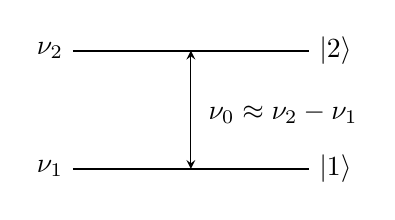
\begin{tikzpicture}
              \draw[thick] (0,0)--(3,0) node[right] {$|1\rangle$};
               \draw[thick] (0,1.5)--(3,1.5) node[right] {$|2\rangle$};
                \draw[stealth-stealth] (1.5,0)--(1.5,1.5);
                \node[right] at (1.6,0.7){$\nu_{0} \approx \nu_{2}-\nu_{1}$};
                \node [left] at (0,0) {$\nu_{1}$};
                \node [left] at (0,1.5) {$\nu_{2}$};
          \end{tikzpicture}
          \label{fig:figure 1}
          
   \end{figure}
\item   \textcolor{blue}{\underline{Absorption profile}}   
\begin{columns}
    
\column {0.4\textwidth}
\begin{figure}
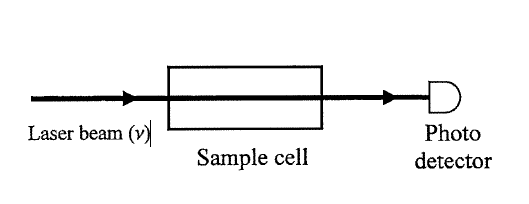
\includegraphics[scale=0.35]{absorption.png}
\end{figure}
\column {0.4\textwidth}
\begin{figure}
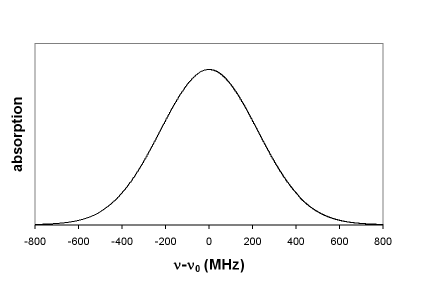
\includegraphics[scale=0.35]{simple.png}
\end{figure}
\end{columns}
\end{itemize}
\tiny{Source: Ghosh, Pradip Narayan - Laser Physics and Spectroscopy (2018, CRC Press)}
\end{frame}
%\begin{block} {Semiclassical approach}
%\end{block}
%\begin{itemize}
 %  \item An atom is considered as quantum mechanical system
  %  \item EM radiation is taken as classical wave
%\end{itemize}
%\begin{block}{Hamiltonian}
%\end{block}
%\begin{itemize}
 %   \item The total Hamiltonian of the system can be written as$$ \mathcal{\hat{H}} = \mathcal{\hat{H}}_0 + \mathcal{\hat{H}}_I $$ $\mathcal{\hat{H}}_0$ is the Hamiltonian for the unperturbed system and $\mathcal{\hat{H}}_I $ is the atom field interaction Hamiltonian.
  %  \begin{eqnarray*}
   %  \mathcal{\hat{H}}_0 &=&\hbar\omega_a|a \rangle \langle a|+\hbar\omega_b|b \rangle \langle b|\\
    % \mathcal{\hat{H}}_I &=& -\frac{\hbar\Omega}{2}(|a \rangle \langle b|e^{-i \omega t}+ |b \rangle \langle a|e^{i\omega t})  
    %\end{eqnarray*}
    %where Rabi frequency,  $\Omega= \mu \frac{E_0}{\hbar}$
%\end{itemize}





%================================================
%                    SAS
%===============================================\section{\textbf{Coherent phenomena in atomic medium }}
\begin{frame}{\textbf{Saturation Absorption Spectroscopy (SAS)}}
\begin{figure}
    \centering
    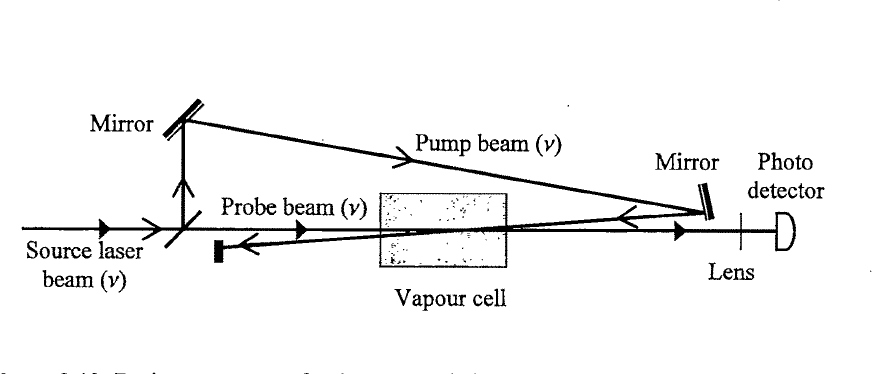
\includegraphics[scale=0.4]{SAS.png}
    \caption{Basic experimental set up for SAS}
    \label{fig:figure 2}
\end{figure}
\begin{itemize}
   % \item Doppler free spectroscopy.
    \item A technique to resolve narrow hyperfine  transition.
   % \item Action of two counter propagating beams creates a sharp dip in velocity distribution curve. 
    \item In 1970, Schawlow and Hansch first developed the technique known as laser-saturated absorption spectroscopy. 
\end{itemize}

\tiny{Source: Ghosh, Pradip Narayan - Laser Physics and Spectroscopy (2018, CRC Press)}
\end{frame}

%******************************************************
\begin{frame}{\textbf {SAS in 2-level atomic system}}
\begin{figure}
     \centering
     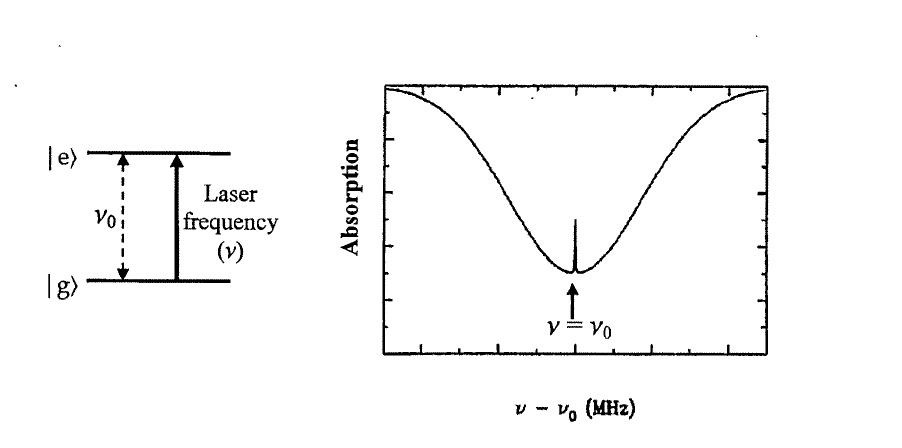
\includegraphics[scale=0.4]{SAS twolevel.png}
     \caption{Absorption spectrum for 2-level atomic system under SAS configuration.}
     \label{fig:figure 3}
 \end{figure}
 \begin{itemize}
\item Doppler free spectroscopy.
 \item Action of two counter propagating beams creates a sharp dip in velocity distribution curve.
 \end{itemize}
 \tiny{Source: Ghosh, Pradip Narayan - Laser Physics and Spectroscopy (2018, CRC Press)}
\end{frame}

\begin{frame}{SAS in 3-level atomic system }
\centering
\textcolor{blue}{\underline{\textbf{Crossover Resonance}}}
\begin{figure}
    \centering
    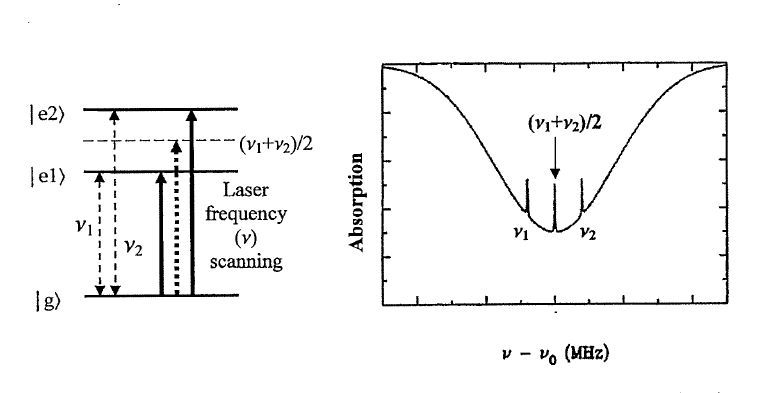
\includegraphics[scale=0.4]{SAS threelevel.png}
    \caption{Probe absorption spectrum for 3-level atom under SAS configuration.}
    \label{fig:enter-label}
\end{figure}
%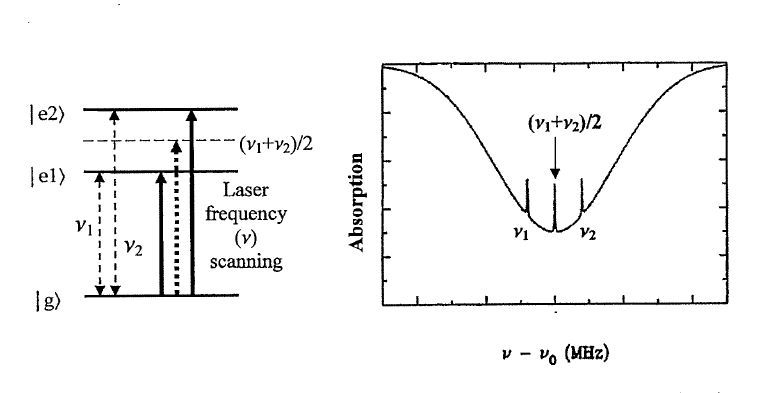
\includegraphics[scale=0.5]{SAS threelevel.png}
%\caption{}
\begin{itemize}
   \item Two dips on the left and right side are hyperfine transitions.
   \item Third dip in middle is crossover resonance dip.
  \end{itemize}
\tiny{Source: Ghosh, Pradip Narayan - Laser Physics and Spectroscopy (2018, CRC Press)} 
\end{frame}

%=====================================================
%                      CPT
%=====================================================
\begin{frame}
\begin{center}
    \begin{tcolorbox}[arc=3mm, width= 10cm, colback=blue!10!white, halign= center,]
             \textbf{Coherent optical phenomena in 3 level atomic system }
         \end{tcolorbox}
\end{center}
    
\end{frame}

\begin{frame}{\textbf{Coherent Population Trapping}}
\begin{itemize}
    \item Observed in 3-level system where both pump and probe laser beam acts simultaneously. 
    \item Atomic population get trapped in coherent superposition state of two ground states $|1\rangle$ and $|2\rangle$.
   % \item Observed in 3-level system where both pump and probe laser beam acts simultaneously. 
    \item No absorption takes place from this state in presence of the field.
    %\item CPT occurs when frequency difference between two external beams matches with the separation between two ground state energy level.
    \item First experimentally observed in a 3-level system by Alzetta \textit{et al} in 1976.
    \end{itemize}
  % \begin{figure}
     %  \centering
      % 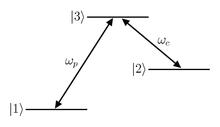
\includegraphics{cpt.jpg}
       %\caption{Lambda ($\Lambda$)-type system}
  % \end{figure}
\end{frame}
\begin{frame}
\begin{figure}
\begin{center}
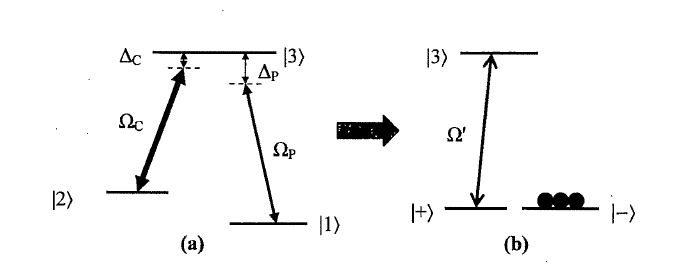
\includegraphics[scale=0.4]{CPT}
\caption{(a) Energy level diagram for 3-level
lambda ($ \Lambda $)-type system. (b) The population is pumped into a superstition state ($ | -\rangle $) of the two ground states. }
\end{center}
\end{figure}
\begin{itemize}
    \item Hamiltonian for 3-level atomic system is given by,
  \begin{equation*}
    H=H_{0}+H_{I} 
\end{equation*}
%atom-laser interaction Hamiltonian,
%\begin{equation}
%  H_I= -\frac{\hbar}{2}[(|1\rangle \langle3| \Omega_p e^{-i\omega_p t} ) + (|2\rangle \langle3| \Omega_c e^{-i\omega_ct})+ C.C.]  
%\end{equation}
\item Eigenstates of H at resonance condition will be as follows:
\begin{eqnarray*}
 |+\rangle = \frac{\Omega_{p}}{\Omega^{'}} |1\rangle + \frac{\Omega_{c}}{\Omega^{'}} |2\rangle  \\
  |-\rangle = \frac{\Omega_{c}}{\Omega^{'}} |1\rangle - \frac{\Omega_{p}}{\Omega^{'}} |2\rangle
\end{eqnarray*}
where $ \Omega^{'} = (\Omega^{2}_{c} + \Omega^{2}_{p})$.
\item The state $|-\rangle$ is nonabsorbing and it is called dark or trapped state.
\end{itemize}
\tiny{Source: Ghosh, Pradip Narayan - Laser Physics and Spectroscopy (2018, CRC Press)}
\end{frame}
%===============================================%
%                    EIT
%=================================================
\begin{frame}{\textbf {Electromagnetically Induced Transparency (EIT)}}
  \begin{itemize}
      \item A quantum mechanical phenomena which alters the optical properties of an atomic medium under the action of resonant electromagnetic field.
      \item Opaque medium exhibits high transparency at resonant frequency.
      \item Quantum destructive interference between 2 excitation pathways leads to nonabsorption of probe field.
      \item EIT was first observed in 3-level Lambda ($\Lambda$) type system.
      
  \end{itemize}
  

\end{frame}

\begin{frame}{\textbf{$\Lambda$-type system }}
\begin{itemize}
    \item \textcolor{blue}{Two ground hyperfine energy levels are coupled to a common excited level via pump and probe laser beam.}
    \vspace{5mm}
    \begin{center}
    \begin{tcolorbox}[width=9cm, colback=yellow!3!white]
     \begin{figure}[ht]
     \centering
      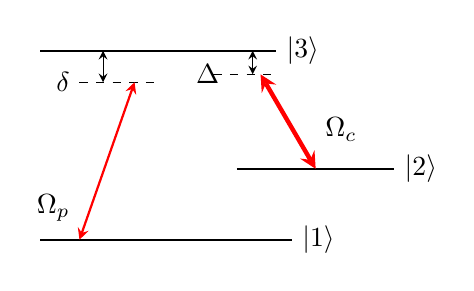
\begin{tikzpicture}
\draw [thick](0,0)--(3,0) node[right] {$|3\rangle$} ;
\draw[thick] (2.5,-1.5) -- (4.5,-1.5) node[right] {$|2\rangle$};
\draw[thick] (0,-2.4)--(3.2,-2.4) node [right]{$|1\rangle$};
\draw[dashed](2.2,-0.3)--(3,-0.3);
\draw[dashed](0.5,-0.4)--(1.5,-0.4);
\draw[stealth-stealth](2.7,-0.3)--(2.7,0)node[left] at(2.4,-0.3) {$\Delta$} ;
\draw[stealth-stealth](0.8,-0.4)--(0.8,0)node[left] at(0.5,-0.4) {$\delta$}  ;
\draw[stealth-stealth,thick,red](0.5,-2.4)--(1.2,-0.4);
\draw[stealth-stealth,ultra thick,red] (3.5,-1.5) --(2.8,-0.3);  
\node [right] at (3.5,-1) {$\Omega_c$};
\node [left] at (0.5,-2) {$\Omega_p$};
 \end{tikzpicture}
     \caption{Lambda ($\Lambda$)- type atom-laser interaction system}
     \label{fig:lambda}
     \end{figure}
     \end{tcolorbox}
     \end{center}
     \end{itemize}
     \end{frame}

     
   \begin{frame}{\textbf{OBEs for 3 level $\Lambda$ type system}}
      \begin{tcolorbox}[colback= blue!5]
          \begin{eqnarray*}
\begin{aligned}
\dot{\tilde{\rho}}_{11}&= \frac{i\Omega_{p}}{2} (\tilde{\rho}_{31} -\tilde{\rho}_{13}) + \Gamma_{21} (\tilde{\rho}_{22} -\tilde{\rho}_{11}) + \Gamma_{31} \tilde{\rho}_{33}\\
\dot{\tilde{\rho }}_{22}&= \frac{i\Omega_{c}}{2} (\tilde{\rho}_{32} -\tilde{\rho}_{23}) - \Gamma_{21} (\tilde{\rho}_{22} -\tilde{\rho}_{11}) + \Gamma_{32} \tilde{\rho}_{33}\\
\dot{\tilde{\rho }}_{33}&= \frac{i\Omega_{p}}{2} (\tilde{\rho}_{13} -\tilde{\rho}_{31}) + \frac{i\Omega_{c}}{2} (\tilde{\rho}_{23} -\tilde{\rho}_{32}) - (\Gamma_{32} + \Gamma_{31}) \tilde{\rho}_{33}\\
\dot{\tilde{\rho }}_{21}&= [ i (\delta - \Delta)-\gamma_{21}]\tilde{\rho}_{21} + \frac{i\Omega_{c}}{2} \tilde{\rho}_{31} - \frac{i\Omega_{p}}{2} \tilde{\rho}_{23}\\
\dot{\tilde{\rho }}_{31}&= [ i \delta - \gamma]\tilde{\rho}_{31} + \frac{i\Omega_{p}}{2} (\tilde{\rho}_{11} - \tilde{\rho}_{33}) + \frac{i\Omega_{c}}{2} \tilde{\rho}_{21}\\
\dot{\tilde{\rho }}_{32}&= [ i\Delta-\gamma]\tilde{\rho}_{32} + \frac{i\Omega_{c}}{2} (\tilde{\rho}_{22} - \tilde{\rho}_{33})+ \frac{i\Omega_{p}}{2} \tilde{\rho}_{12}
\end{aligned}
\end{eqnarray*}
\end{tcolorbox}
\iffalse
$\Delta$ and $\delta$ are the pump and probe detuning respectively.\\
The decay terms are,
%\begin{eqnarray}
$\gamma_{21}=\frac{\Gamma_{21}+\Gamma_{12}}{2}\nonumber$,
$\gamma=\frac{\Gamma_{21}+\Gamma_{31}+\Gamma_{32}}{2} $.
\fi  
   \end{frame} 


\begin{frame}{Analytical solution for OBEs}
%\begin{columns}
  %\column{0.5\textwidth}  

    \begin{center}
    \begin{tcolorbox}[width=7cm,arc=2mm,colback=blue!7 ]
    %\begin{itemize}
    %\item Under weak probe approximation, the solution for OBEs given as,
            \begin{equation}
          \tilde{\rho}_{31}=\frac{-\frac{i\Omega_{P}}{2}}{(\gamma -i\delta)+\frac{\frac{\Omega_{C}^{2}}{4}}{\gamma_{21}-i(\delta-\Delta)}}\nonumber
          \label{eqn obe}
            \end{equation}
%\end{itemize}
            
           \end{tcolorbox}  
           \end{center}
%\column{0.5\textwidth}

\begin{itemize}
%\centering
    \item  {\textcolor{blue}{Probe absorption profile}}
 %  
       \begin{figure}
            \centering
        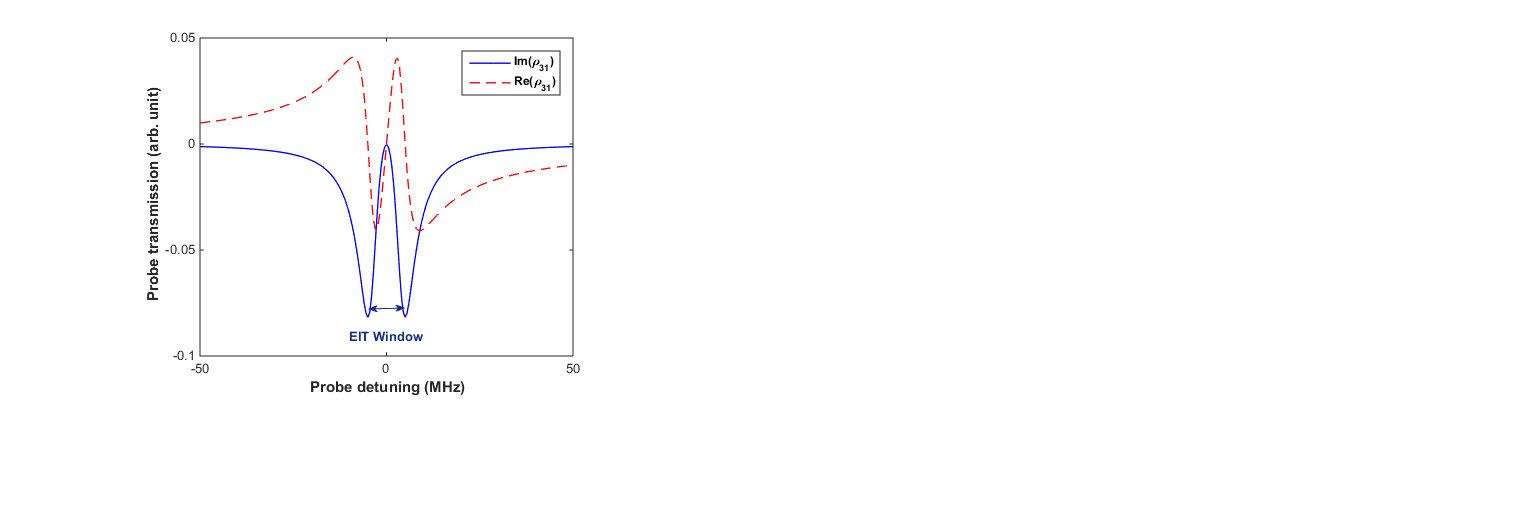
\includegraphics[scale=0.35]{Lambda(Analytical).png}
        \vspace{-1.5cm}
    \caption{Real and imaginary part of $\tilde\rho_{31}$ vs probe detuning ($\delta$) for $\Lambda$-type system }
     \label{fig:lambda_1}
 \end{figure}
   %\end{center}
          
 \end{itemize}
     % \end{column}
%\end{columns}
\end{frame}

\begin{frame}
 % \begin{center}
%\textcolor{blue}{\underline{ Intensity Distribution of Gausian and LG beam}}
%\end{center} 
\begin{columns}
        
 \column {0.5\textwidth}
    \begin{itemize}
        \item \textcolor{blue}{\textbf{V-type system}}
    \end{itemize}
    \begin{figure}
        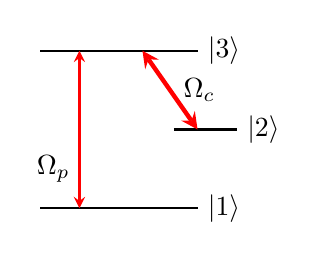
\begin{tikzpicture}
\draw [thick](0,0)--(2,0) node[right] {$|3\rangle$} ;
\draw[thick] (1.7,-1) -- (2.5,-1) node[right] {$|2\rangle$};
\draw[thick] (0,-2)--(2,-2) node [right]{$|1\rangle$};
\draw[stealth-stealth, thick,red](0.5,-2)--(0.5,0);
\draw[stealth-stealth,ultra thick,red] (2,-1) --(1.3,0);  
\node [right] at (1.7,-0.5) {$\Omega_c$};
\node [left] at (0.5,-1.5) {$\Omega_p$};
 \end{tikzpicture}
 \end{figure}
 \begin{figure}
 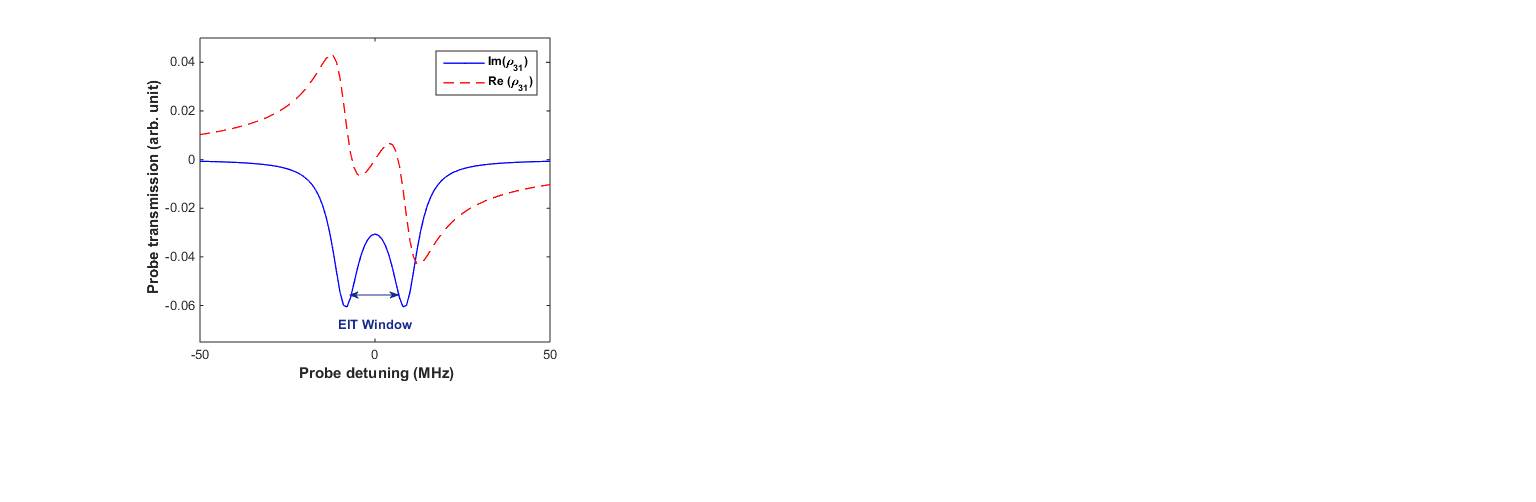
\includegraphics[scale = 0.3]{V(Analytical).png}
 \end{figure}
  %  \includegraphics[scale = 0.28]{lg_int_1}
    %\vspace{0.5cm}
\column{0.5\textwidth}
  \begin{itemize}
      \item \textcolor{blue}{\textbf{Cascade type system}}
  \end{itemize}
    \begin{figure}
     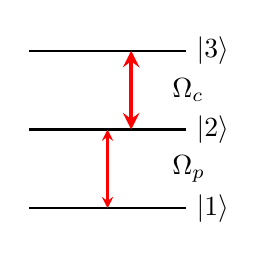
\begin{tikzpicture}
\draw [thick](0,0)--(2,0) node[right] {$|3\rangle$} ;
\draw[thick] (0,-1) -- (2,-1) node[right] {$|2\rangle$};
\draw[thick] (0,-2)--(2,-2) node [right]{$|1\rangle$};
\draw[stealth-stealth, thick,red](1,-2)--(1,-1);
\draw[stealth-stealth,ultra thick,red] (1.3,-1) --(1.3,0);  
\node [right] at (1.7,-0.5) {$\Omega_c$};
\node [right] at (1.7,-1.5) {$\Omega_p$};
 \end{tikzpicture}
 \end{figure}
 \begin{figure}
    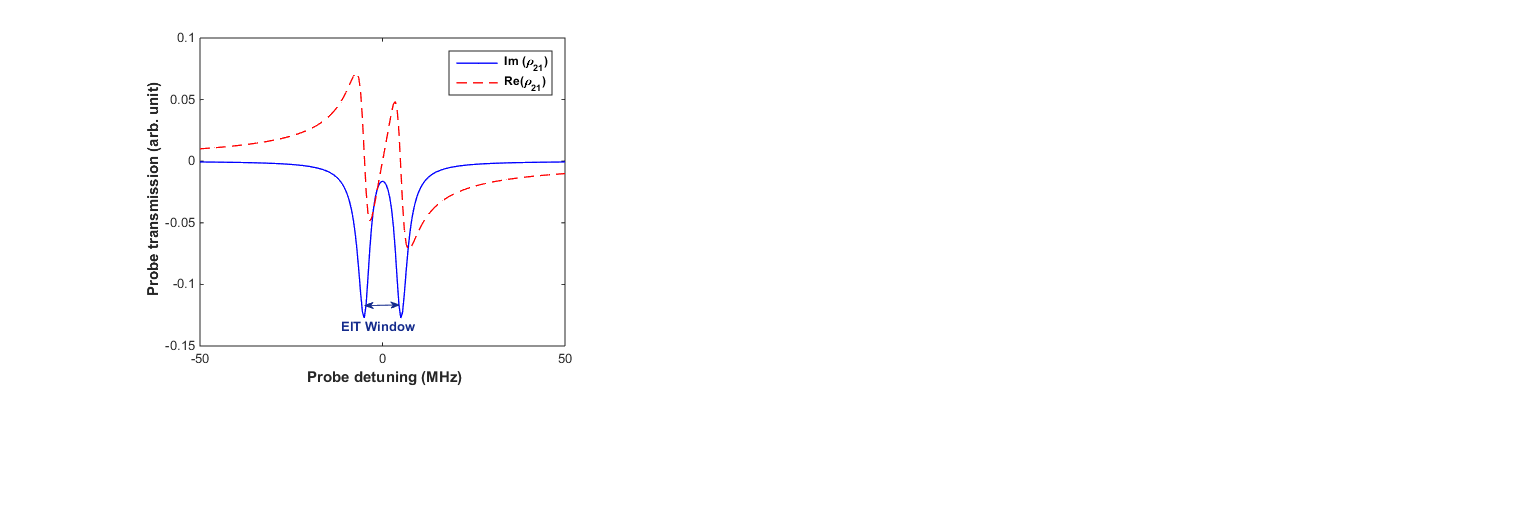
\includegraphics[scale = 0.3]{Cascade(Analytical).png}
    \end{figure}
    \end{columns}   
\end{frame}

%==============================================
%                NIM
%==============================================
   \begin{frame}{\textbf{Negative Index Material (NIM)}}
   \begin{figure}
       \centering
       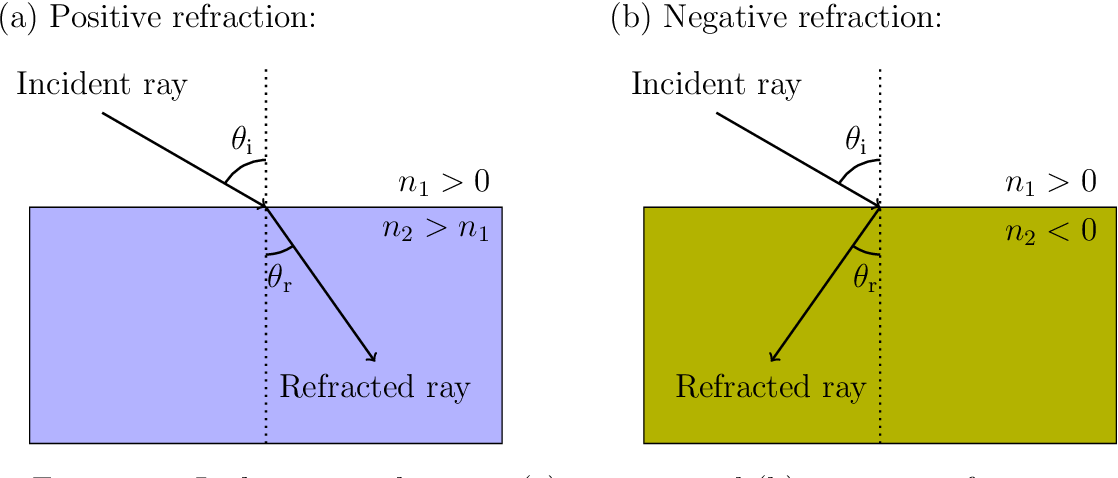
\includegraphics[scale=0.2]{NRI (MM).png}
       \caption{Positive and negative index material.}
       \label{fig:enter-label}
       \vspace{2mm}
       \tiny{Source: \url{https://www.semanticscholar.org/paper/The-Application-of-Negative-Refractive-Index-to-mm-Mohamed/57d7f5af72043c0e8d0e6d68ca7d7a89d37f6da9}.}
   \end{figure}
   \begin{itemize}
       \item An engineered material in which refractive index of material is negative.
        \end{itemize}
 \end{frame}

 \begin{frame} {NIM}
\begin{figure}
    \centering
    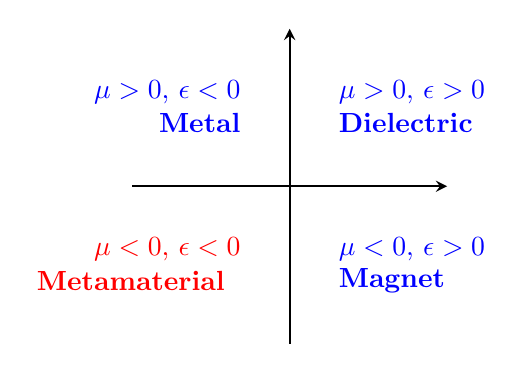
\begin{tikzpicture}
     \draw [thick,-stealth](0,0)--(4,0);
     \draw [thick,stealth-](2,2)--(2,-2);
    \node [blue,right] at (2.5,1.2) {$\mu>0$, $\epsilon >0$};
    \node [blue,right] at (2.5,0.8) {\bf{Dielectric}} ;
     \node [blue,left ] at (1.5,1.2) {$\mu>0$, $\epsilon <0$};
    \node [blue,left] at (1.5,0.8) {\bf{Metal}} ;
     \node [red,left] at (1.5,-0.8) {$\mu<0$, $\epsilon <0$};
    \node [red,left] at (1.3,-1.2) {\bf{Metamaterial}} ;
     \node [blue,right] at (2.5,-0.8) {$\mu<0$, $\epsilon >0$};
    \node [blue,right] at (2.5,-1.2) {\bf{Magnet}} ;
    \end{tikzpicture}
    \caption{Permittivity and permeability diagram }
\end{figure}    

 \begin{itemize} 

     \item Both permittivity and permeability of the material is negative.
       \item Wave vector and Poynting vector are antiparallel.
        \end{itemize}
 \end{frame}

%===================================================
%                     SPP
%===================================================
%\iffalse
\begin{frame}{\textbf{Surface Plasmon Polariton}}
\begin{figure}
    \centering
    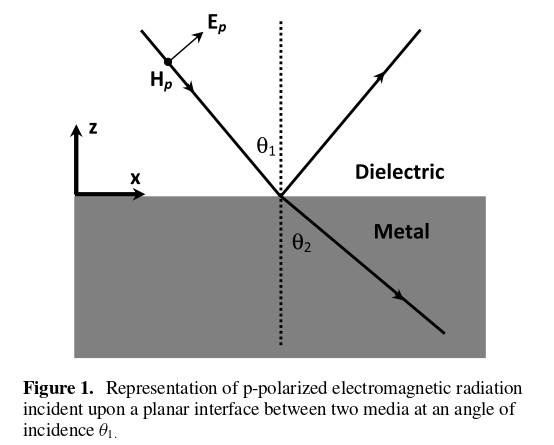
\includegraphics[scale=0.6]{zhang2012 (1)-3_cropped_page-0001.jpg}
\end{figure}
\begin{itemize}
   \item SPP is electromagnetic wave present at the interface between metal and dielectric.
   \item Surface electromagnetic wave consist of  surface charges.
   \item When a p-polarized light is incident upon a metal surface at an angle beyond $\theta_{c}$ (critical angle), a spatially decaying field (evanescent wave) propagates in a direction normal to the surafce.
   \item At critical angle the decay length is infinite and beyond critical angle it is order of few wavelength.
\end{itemize}
 \tiny{Zhang et al. J.Phys.D: Appl. Phys. 45 (2012) 113001 (19pp)}   
\end{frame}

\begin{frame}{\textbf{EIT in SPP system}}
 \begin{figure}
     \centering
     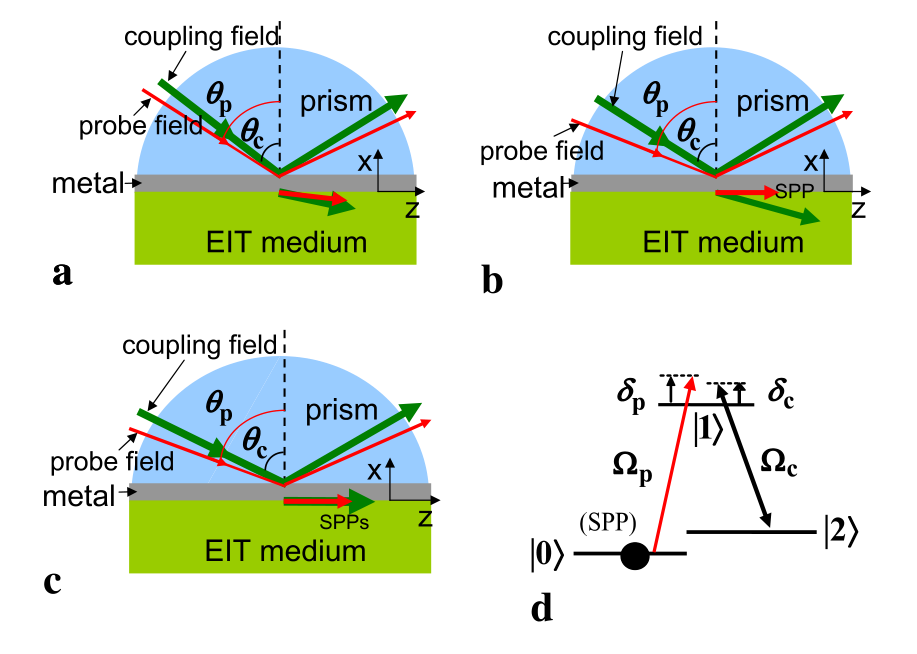
\includegraphics[scale=0.7]{spp_angle_diagram.png}
\end{figure}
\begin{itemize}
 \item EIT can be used for coherent control of light by excitation of SPP.
     \item EIT based SPR system consist of three layers among which the third level acts as EIT medium.
     \item In a SPR system the pump and probe beam can be considered as follows
     \begin{itemize}
         \item The coupling or pump field is freely propagating field and the probe field is a SPP. 
         \item Or the coupling field is a SPP field.
     \end{itemize}
     \item Choice of coupling field leads to different frequency spectra for reflectivity of probe beam.
 \end{itemize} 
 \tiny{Du \textit{et al.}Physical Review A, 91(1):013817, 2015.}
\end{frame}
%\fi
%===============Literature Survey=====================%
\section{\textbf{Literature survey}}
\begin{frame}
\begin{center}
    \begin{tcolorbox}[arc=3mm, width= 10cm, colback=blue!10!white, halign= center,]
             \textbf{Literature Survey }
         \end{tcolorbox}
\end{center}
\end{frame}

%    =========COP in atomic medium============    %

 \begin{frame}{Coherent optical phenomena (CPT and EIT)}
 \begin{columns}
    \begin{column}{0.5\textwidth}
        \begin{itemize}
            \item In \textcolor{blue}{1976}, Alzetta \textit{et al.} first experimentally observed CPT.
         \item Three black lines in fluorescence of Na atoms were detected.
        \end{itemize}
    \end{column}
    \begin{column}{0.5\textwidth}
       % \rule{\textwidth}{0.75\textwidth}{G}
       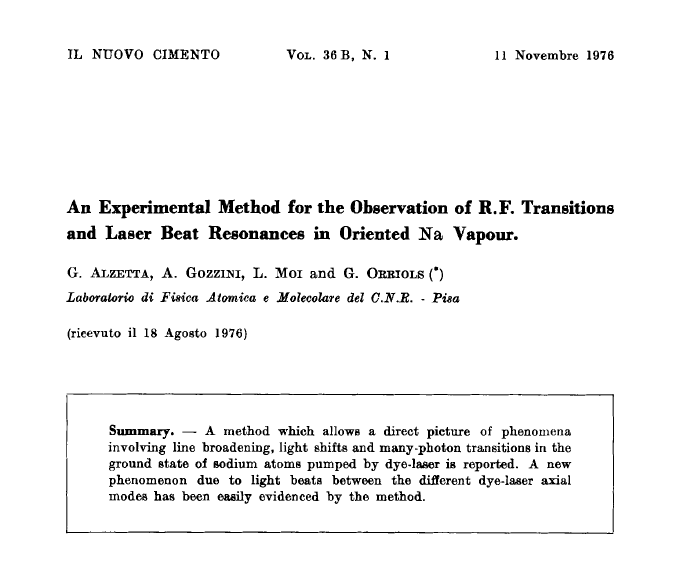
\includegraphics[scale = 0.3]{alzeta}
    \end{column}
\end{columns}
\end{frame}  

\begin{frame}
 \begin{center}
      \textcolor{red}{\underline{ \textbf{1976-1989}}}
      \end{center}
     \begin{itemize}
         \item  In \textcolor{blue}{ 1976}, Arimondo gave the theoretical analysis of coherent phenomena in 3-level system.
         \item In \textcolor{blue}{1984}, Bright reviewed the use of EM field to create transparency.
         \item In \textcolor{blue}{1986}, Kocharovskaya and Khanin predicted the population trapping in two lower levels of $\Lambda$ configuration  .
     \item Also the foundations of EIT were laid by them in \textcolor{blue}{1988}.
\item In \textcolor{blue}{1989}, Harris independently observed EIT. 
     \end{itemize}
     \end{frame}
% \iffalse    
\begin{frame}
\begin{columns}
\column{0.5\textwidth}
 \begin{itemize}
 
        % \item The name EIT was first proposed by Harris.
         \item In \textcolor{blue}{1991}, Harris \textit{et al.} first experimentally demonstrated EIT.
       % \item  In their paper the resonantly enhanced non-linear susceptibility based on EIT was proposed.
\item  This experiment was carried out in a $\Lambda$ scheme in Strontium vapour using pulsed lasers.
\item  Result shows that the transmittance of the probe field, could be increased from $ e^{-20} $ to $ e^{-1} $.
\item  They pointed out the importance of the quantum interference in this increment. 
\item  For no interference process present, the transmittance would only have increased to $ e^{-7} $.
\end{itemize}
\column{0.4\textwidth}
    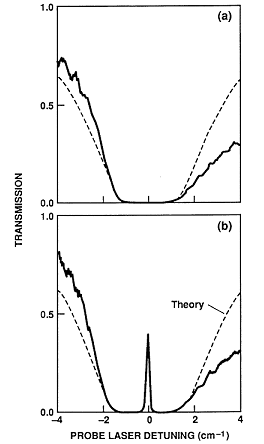
\includegraphics[scale=0.5]{1steit.png}
    
\end{columns}
\end{frame}

\begin{frame}
    
 \begin{center}
      \textcolor{red}{\underline{ \textbf{1990-1999}}}
 \end{center}
    \begin{itemize}
        \item In the same year, Field \textit{et al.} first observed EIT in a collisionally broadened resonance transition of $Pb$ vapour.
       \item In \textcolor{blue}{1992},  Kasapi \textit{et al.} experimentally  demonstrated EIT in a cascade $\Xi$-type in Lead vapour.
       \item In \textcolor{blue}{1994}, Eberly and his group  first observed spatial evolution of dressed field pulses. This result provided the information of EIT propagation.
 \end{itemize}
\end{frame}
       \begin{frame}
       \begin{columns}
       \column{0.4\textwidth}
       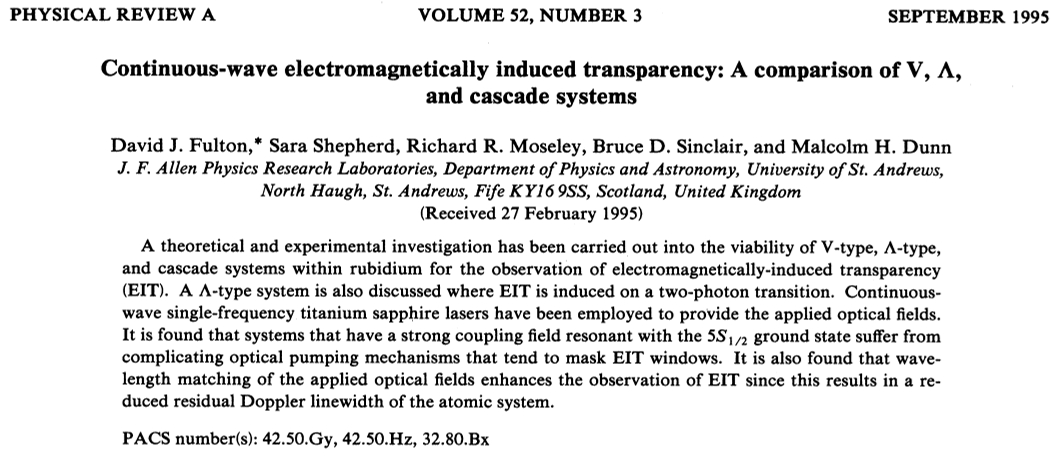
\includegraphics[scale=0.35]{fulton1995-1-1.jpg}
       \column{0.4\textwidth}
       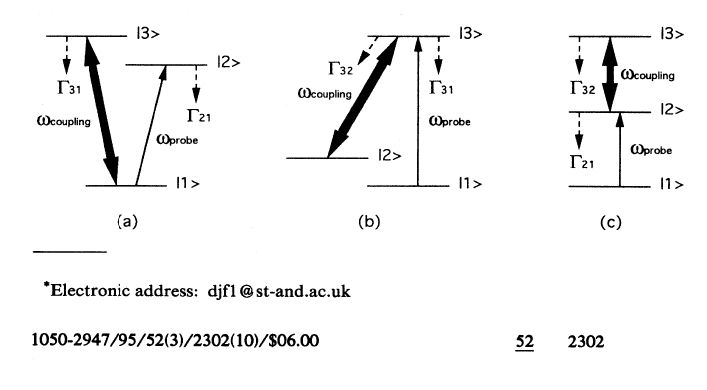
\includegraphics[scale=0.45]{pdfresizer.com-pdf-crop_page-0001.jpg}
       \end{columns}
           \begin{itemize}
      \item In \textcolor{blue}{1995}, Fulton \textit{et al.} conducted theoretical and experimental investigations on continuous-wave EIT in $\Lambda$, $\V$ and $\Xi$-type system in Rb atom.
      \end{itemize}
\end{frame}
 %\fi     
      \begin{frame}
      \begin{itemize}
          \item  In \textcolor{blue}{1996}, Kasapi \textit{et al.} applied EIT to isotope discrimination by adjusting the intensity of a coupling laser.
          \item In \textcolor{blue}{1997}, Hopkins \textit{et al.} investigated EIT in laser cooled medium.
      \item In \textcolor{blue}{1998}, Azim \textit{et al.}proposed a method to measure photon statistics of a quantized radiation field in an EIT set-up.
     \item In the year \textcolor{blue}{1999}, 
     \begin{itemize}
         \item Boon and his group experimentally observed of transparency on a transition in the blue spectral region in a V-type system.
         \item Ying-Cheng Chen \textit{et al.} experimentally detected fast and slow light using EIT.
         \item Hau \textit{et al.} reported an experimental demonstration of EIT in ultra cold Na atoms, where optical pulses propagated at twenty million times slower than the speed of light in vacuum.
         \end{itemize}
      \end{itemize}

    \end{frame}
    \begin{frame}
    \begin{center}
        \textcolor{red}{\underline{\textbf{2000-2009}}}
    \end{center}
    \begin{itemize}
\item In \textcolor{blue}{2000}, Entin \textit{et al.} experimentally demonstrated non degenerate four-level N-type scheme to observe EIT at the $^{87}Rb$ $D_{2}$ line.
\item In \textcolor{blue}{2001},
\begin{itemize}
    \item Badger and his group investigated the role of hyperfine structure in EIT by studying the $5S_{1/2} - 5P_{3/2} - 5D_{3/2,5/2}$ cascade ($\Xi$)-type system in $^{85}Rb$ and $^{87}Rb$.
    \item Chen \textit{et al.} first reported the observation of narrow and high contrast spectra in a $\Lambda$-type configuration.
    \item In \textcolor{blue}{2001}, Wang  and his group experimentally investigated EIT in a multi-level cascade ($\Xi$) type system of cold $^{85}Rb$ atoms and proposed Kerr nonlinearity in EIT windows.
 
   \item In this year , Dogariu and Kim proposed dispersive properties if EIT.
   \end{itemize}

\item In \textcolor{blue}{2002}, Kozuma and his co workers reported an experimental investigation of group velocity reduction and light storage.
\end{itemize}
\end{frame}

\begin{frame}
\begin{itemize}
\item In \textcolor{blue}{2004},  Carvalho led group measured the dependence of the linewidth of an EIT resonance on the angle between coupling and probe beams.

\item In \textcolor{blue}{2005}, Chakrabarti \textit{et al.} reported the additional absorption enhancement peak in a $\Lambda$-type system due to velocity selective optical pumping along with EIT.
\item In \textcolor{blue}{2006}, Wang observed two-photon transparency.
\end{itemize}
\end{frame}

%cccccccccccccccccccccccccccccccccccccccccccccccccccc
%\iffalse
\begin{frame}
\begin{center}
    \textcolor{red}{\underline{\textbf{Other type of atom-laser coupling scheme}}}
\end{center}

\begin{itemize}
    \item \textcolor{blue}{Inverted Y type system :} Yan \textit{et al.} explored EIT in an inverted-Y system of interacting cold atoms.
   
    %\item \textcolor{blue}{Tripod- type system :}
    \item \textcolor{blue}{$N$ level system :} In \textcolor{blue}{2008}, Anton \textit{et al.} delved into optical switching in a five level atom through EIT. Chen \textit{et al.} and Kong \textit{et al.} explored the optical properties of an N-type system in Doppler broadened multilevel atomic media.
    % \end{itemize}
   % \iffalse
    \item \textcolor{blue}{Rydberg EIT :} Naber \textit{et al.} investigated EIT with Rydberg atoms across the Breit-Rabi regime. Tian \textit{et al.}  modeled EIT in a Y system with a single Rydberg state. Kara \textit{et al.} studied Rydberg interaction induced enhanced excitation in thermal atomic vapor.
  \end{itemize}
 \end{frame}
 \fi
%    =========MM & SPP===============   %          
    \begin{frame}{Metamaterial and EIT}
    \begin{itemize}
        \item In \textcolor{blue}{1967}, Veselago first predicted about negative index material.
        \item In \textcolor{blue}{1999}, Sir John Pendry first paved the way to develop a NIM. He showed that a sub wavelength metalic structure called split ring resonator can produce negative permeability at certain frequency.
        \item In \textcolor{blue}{2000}, Smith \textit{et al.} demonstrated the first metamaterial with a negative refractive index at microwave frequencies using split-ring resonators (SRRs) and wire structures.
        \item \textcolor{blue}{2003-2005}: During this time researcher focused on developing NIM within various frequency range.
        \begin{itemize}
            \item  Yan \textit{et al.} achieved negative permeability at 1 THz.
         \item An alternative technique,used by Zhang \textit{et al.} led to achieve resonance frequency up to 60THz.

         \item Linden and his group found that magnetic response of a material can be achieved at 85 THz. 
        \end{itemize}
        
    \end{itemize}
       \end{frame}
       \begin{frame}
       \begin{itemize}
           \item \textcolor{blue}{2005-2007}: Several theoretical and experimental works carried out to achieve negative refractive index at optical wavelength.
           \item In \textcolor{blue}{2008}, Zhang \textit{et al.} first designed EIT metamaterial with a working frequency of 428.4 THz.\footnote{ Shuang Zhang, Dentcho A Genov, Yuan Wang, Ming Liu, and Xiang Zhang. Physical review letters, 101(4):047401, 2008.}
           \begin{figure}
           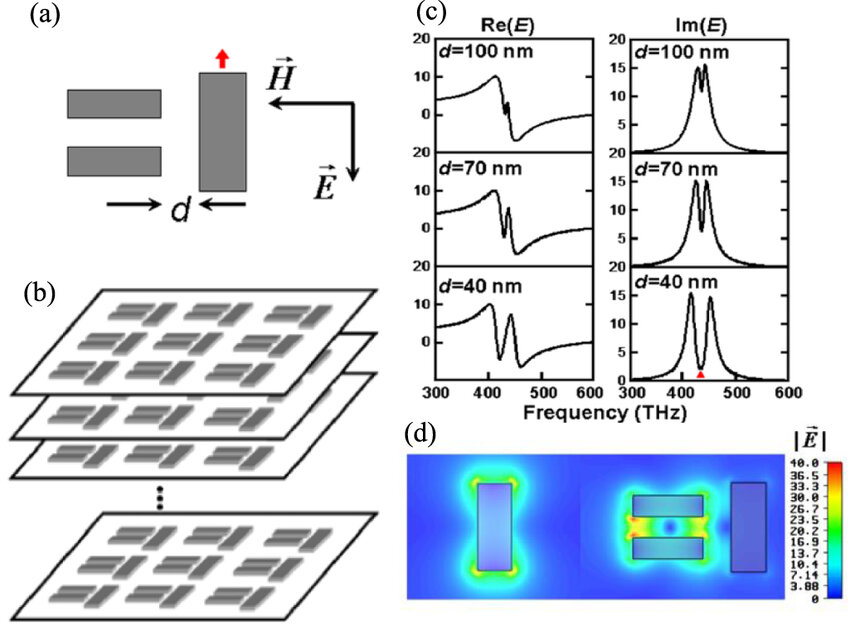
\includegraphics[scale=0.6]{EIT MM (Zhang et al).png}
           \end{figure}
         %  \item In \textcolor{blue}{2009}, Chiam \textit{et al.} and Liu \textit{et al.} demonstrated EIT in palnar metamaterial.
           \item In next decade significant progress has been made in the field of EIT in meatmaterial. In this era, a lot of microstructures and methods to realize plasmonic EIT effects have been proposed. 
              %As long as the polarization state of incident E-field is changed, the number of transparent windows can be controlled, which possesses the advantages of adjustable amplitude and resonance wavelength.

       \end{itemize}
   \end{frame}
%========================================================
   \begin{frame}{SPP}
   \begin{itemize}
      \item SPPs were first observed by Wood in \textcolor{blue}{1902}. He found
        unexplained features in optical reflection measurements on metallic gratings
      \item The term \textbf{plasmon} was first introduced by Pines in \textcolor{blue}{1956}.
      \item In the same year, Fano first used the term \textbf{polariton} for the coupled oscillation of bound electron.
      \item  Ritchie in \textcolor{blue}{1957} investigated electron energy losses in thin films and gave first theoretical description of\textbf{ surface plasmons}. It was found that plasmon modes could exist near the surface of metals. %then, he described the anomalous behaviour of
%metal gratings in terms of surface plasmon resonances excited
%on the gratings
      \item In \textcolor{blue}{1968} Otto and Kretschmann  first proposed optical excitation of surface plasmons on metal films in their work differently.
      \item Surface plasmon properties
       of gold and silver were described by Kreibig
        and Zacharias in \textcolor{blue}{1970}.
        \item In \textcolor{blue}{1974} Cunningham and co-workers introduced the term surface plasmon polariton (SPP).
    \end{itemize} 
 \end{frame}
    
 \begin{frame}{SPP}
     \begin{itemize} 
    \item In \textcolor{blue}{1997}, Barren \textit{et al.} studied the propagation of surface plasmon polaritons on textured surfaces, specifically on a grating surface. 
\item In \textcolor{blue}{1998}, Kano \textit{et al.} calculated the electric field intensity distribution on a silver surface which is caused by the excited surface plasmon polaritons. 
\item In the same year, elastic scattering of SPP was first modeled by Bozhevolnyi \textit{et al.} by considering isotropic point like scatterers whose responses to the incident SPP field are phenomenologically related to their effective polarizabilities.

%\item In\textbf{2002}, Ditlbacher \textit{et al.} reported the experimental realization of highly efficient optical elements built up from metal nanostructures to manipulate surface plasmon polaritons propagating along a polymer interface.\\
\item In \textcolor{blue}{2003}, near field imaging of scattering, reflection, interference and localization of surface polaritons are reviewed by  Zayats and Smolyaninov.
\end{itemize}
\end{frame}

\begin{frame}{SPP}
\begin{itemize}
\item In \textcolor{blue}{2004}, Krenn and Weeber investigated various properties of SPP such as propagation length, mode field profile and reflection or scattering at metal dielectric interfaces. 

%\item In \textbf{2005}, Andre \textit{et al.} presented an overview of recent theoretical and experimental work on the control of the propagation and quantum properties of light using EIT in atomic ensembles. They provided the techniques for the generation and storage of few photon quantum-mechanical states of light as well as novel approaches to manipulate weak pulses of light via enhanced nonlinear optical processes.\\


    \item  In \textcolor{blue}{2010}, Lu \textit{et al.} showed that
%not only localized SSPs but also 
magnetic plasmon resonance play a vital role in plasmonic EIT. %Their interaction was investigated in detail by analyzing the phase evolution of the induced electromagnetic fields in nanoscale volume, which is rendered by the unique near-field properties.\\

%Chen \textit{et al.} in \textbf{2011}, have explored a coupling system structure consisting of cross-slit metallic photonic crystals and dielectric photonic crystals embedded in a background material to achieve polarization independent plasmon induced transparency.\\
\end{itemize}
\end{frame}
 \begin{frame}
 \begin{itemize}    
 \item In \textcolor{blue}{2015}, Du \textit{et al.} first proposed a way to excite SPPs resonantly by lights without using any coupler and a surface-plasmon-resonance (SPR) system.

 %which can be simply composed by a metal film and a bottom medium whose real part of permittivity is less than unity.
\item In the same year Meng \textit{et al.} theoretically studied EIT in reflection spectra of V-type system at the gas-solid interface. In addition to finding a narrow dip arising from the EIT effect, they also explored the other particular saturation effect induced by pump field, which does not exist in $\Lambda$ or $\Xi$ -type system.
\end{itemize}
\end{frame}

%############################################
\begin{frame}{SPP}
\begin{itemize}
\item Asgarnezhad \textit{et al.} in \textcolor{blue}{2017} investigated the possibility of the direct excitation of surface polaritons (SPs) by the free-space laser fields at the interface of negative-index metamaterial (NIMM) layer and a bottom layer of cold double $\Lambda$-type atomic medium. 
%The giant field enhancement together with suppressed ohmic loss of the NIMM layer in a wide transparency window of a double EIT, results in the SPs generation.\\
\item \textcolor{blue}{2018 :} In the following year, the same group investigated the excitation and propagation of the surface polaritonic rogue waves by proposing a coupler free optical waveguide that consists of a transparent layer, middle negative index metamaterial layer and bottom layer of the cold four level atomic medium. 
%In this planar optical waveguide, a giant controllable Kerr nonlinearity is achieved by sufficient field concentration and a proper set of intensities and detunings of the driven laser fields.\\
   \end{itemize}
\end{frame}
%##########################################
  % \begin{frame}{Refferences}
   \begin{frame}[allowframebreaks]{References}
\begin{thebibliography}{21}
\bibitem{int1}C. Cohen-Tanoudji, J. Dupont-Roc and G. Grynberg, \textit{Atom-photon Interactions: Basic Processes and Applications} (Wiley-VCH Verlag GmbH and Co. KGoA, Weinheim) (2004).
\bibitem{int2}W. Demtroder, \textit{Laser Spectroscopy: Basic Concept and Instrumentations} (Springer-Verlag,  $3^{rd}$ Edition) (2003)
\bibitem{int3}Ficek Z. and Swain S 2005 \textit{Quantum Interference and Coherence: Theory and Experiments} Vol 100 (New York: Springer)
\bibitem{int4}U. Fano, \textit{Phys. Rev}, \textbf{124}, 1886(1961)
\bibitem{int5}G. Alzetta \textit{et al.}, \textit{Nuovo Cimento Soc. Ital. Fis.} \textbf{B 36B}, 5 (1976).
\bibitem{int6}E. Arimondo \textit{et al.}, \textit{Lett. Nuovo Cimento} \textbf{17}, 333 (1976)
\bibitem{int7}H. R. Gray \textit{et al.}, \textit{Optics Letters} \textbf{3}, 6 (1978)
\bibitem{int8}Arimondo E 1996 \textit{Prog. Opt.} \textbf{33} 257
\bibitem{int9}Imamogu A and Harris S E \textit{Opt. Lett.} \textbf{14} 1344
\bibitem{int10}Boller K-J, Imamoglu A and Harris S E 1991 \textit{Phys. Rev. Lett.} \textbf{66} 2593
\bibitem{int11}Harris S E 1997 \textit{Phys. Today} \textbf{50} 36
\bibitem{int12}Marangos J P 1998 \textit{J. Mod. Opt.} \textbf{45} 471
\bibitem{int13}Fulton D J, Shepherd S, Moseley R R, Sinclair B D and Dunn M H 1995 \textit{Phys. Rev. A} \textbf{52} 2302

\bibitem{veselago1967electrodynamics} Veselago Viktor G, 1967 \textit{Usp. fiz.nauk} \textbf{92} 517
  %number={7},517,
\bibitem{pendry2000negative}
  %title={Negative refraction makes a perfect lens},
  Pendry et al \textit{Physical review letters} \textbf{85} 3966 (2000

%@article{pendry1999magnetism,
%  title={Magnetism from conductors and enhanced nonlinear phenomena},
 % author={Pendry, John B and Holden, Anthony J and Robbins, David J and Stewart, WJ},
 % journal={IEEE transactions on microwave theory and techniques},
 % volume={47},
  %number={11},
 % pages={2075--2084},
 % year={1999},
 % publisher={IEEE}

%@article{shelby2001experimental,
 % title={Experimental verification of a negative index of refraction},
%  author={Shelby, Richard A and Smith, David R and Schultz, Seldon},
  %journal={science},
 % volume={292},
 % number={5514},
 % pages={77--79},
 % year={2001},
 % publisher={American Association for the Advancement of Science}

  

%%%%%%%%%%%%%%%%%%%%%%%%%%%%%%%%%%%%%%%%%%%%%%%%%%%%%%%%%%%%%
%\iffalse
\bibitem{eitdensity3}H.R. Hamedi \textit{et al.}, \textit{Optics Communications} \textbf{311}, 261–265 (2013)
\bibitem{eitkumar}Kumar \textit{et al.}, \textit{Physical Review A} \textbf{79}, 063821 (2009)
\bibitem{eityan}Dong Yan \textit{et al.}, \textit{Physical Review A} \textbf{86}, 023828 (2012)
\bibitem{eitqi}Jianbing Qi, \textit{Physica Scripta} \textbf{81}, 015402 (8pp) (2010)
\bibitem{eitosma} K.I. Osman \textit{et al.}, \textit{Eur. Phys. J. D} \textbf{54}, 119–130 (2009)
\bibitem{eitkou}Jun Kou\textit{et al.}, \textit{Optics Communications} \textbf{284}, 1603–1607 (2011)
\bibitem{eitliu}J.B. Liu \textit{et al.}, \textit{Journal of Modern Optics} \textbf{56}, 16 (2009)
\bibitem{eitgh}Ghosh \textit{et al.}, \textit{Journal Of Physics B} \textbf{49}, 195401 (14pp) (2016)
\bibitem{eitaton}M.A. Antón \textit{et al.}, \textit{Optics Communications} \textbf{281}, 6040–6048 (2008)
\bibitem{eitchen}Chen \textit{et al.}, \textit{Journal Of Physics B} \textbf{42}, 065506 (10pp) (2009)
\bibitem{eitko}L.B. Kong \textit{et al.}, \textit{Optics Communications } \textbf{269 }, 362–369 (2007)
\bibitem{eitwu}Wu \textit{et al.}, \textit{EPL} \textbf{94}, 64005 (2011)
\bibitem{eitgolu}Yu.M. Golubev \textit{et al.}, \textit{Optics Communications } \textbf{278 }, 350–362 (2007)
\bibitem{naber}Julian B. Naber \textit{et al.}, \textit{SciPost Phys.} \textbf{2}, 015 (2017)
\bibitem{tian}Xue-Dong Tian \textit{et al.}, \textit{Optics Communications } \textbf{345}, 6–12 (2015)
\bibitem{silva}F. Silva \textit{et al.}, \textit{Physical Review A} \textbf{64}, 033802 (2001)
\bibitem{ima}A. Imamoglu, \textit{Physical Review Letters} \textbf{89}, 16 (2002)
%\bibitem{oam1}Allen, L.\textit{et al.}, \textit{Phys.Rev.A} \textbf{45}, 8185–8189(1992).
\iffalse
\bibitem{sas1}P. Meystre and M Sargent III, \textit{Elements of Quantum Optics} (Springer-Verlag, New Delhi) (2006).
\bibitem{sas2}D. Meschede, \textit{Optics, Light and Lasers} (WILEY-VCH Verlag GmbH and Co.) (2007).
\bibitem{sas3}D.W. Preston, \textit{Amer. J. Phys.} \textbf{64}, 1432 (1996).
\bibitem{sas4}K.B. MacAdam, A. Steinbach and C. Wieman, Amer. \textit{J. Phys.} \textbf{60}, 1098 (1992).
\bibitem{sas5}C.E. Wieman and D. Preston, \textit{“Doppler-free saturated absorption spectroscopy”},
Advanced Optics Laboratory,
\textit{http://optics.colorado.edu/~kelvin/classes/opticslab/LaserSpectroscpy6.doc.pdf}
\bibitem{sas6}W.E. Lamb, Jr.,\textit{ Phys. Rev. } \textbf{134}, 1429 (1964).
\bibitem{sas7}\textit{Saturated Absorption Spectroscopy}, Advanced Physics Laboratory, University of
Florida and the References therein.
\bibitem{sas8} Ghosh, Pradip Narayan \textit{Laser Physics and Spectroscopy}(2018) CRC press
\bibitem{cpt1}J.P. Marangos, \textit{J. Mod. Opt.} 45, 471 (1998).
bibitem{eit4}0. A. Kocharovskaya \textit{et al.}, \textit{Zh. Eksp. Teor. Fiz.} \textbf{90}, 1610-1618 (1986)
\bibitem{eit5}O. A. Kocharovskaya \textit{et al.}, \textit{JETP Letters} \textbf{48}, 630-634 (1988)
\bibitem{eit6}S. E. Harris, \textit{Physical Review Letters} \textbf{62}, 1033-1036 (1989).
\bibitem{eit7}S. E. Harris \textit{et al.}, \textit{Physical Review Letters} \textbf{64}, 10 (1990)
\bibitem{eit8}K. J. Boiler \textit{et al.}, \textit{Physical Review Letters} \textbf{66}, 20 (1991)
\bibitem{eit9}J. E. Field \textit{et al.}, \textit{Physical Review Letters} \textbf{67}, 22 (1991)
\bibitem{eit10}Marian O. Scully, \textit{Physical Review Letters} \textbf{67}, 14 (1991)
\bibitem{eit11}S. E. Harris \textit{et al.}, \textit{Physical Review A} \textbf{46}, 1 (1992)
\bibitem{eit12}Eberly \textit{et al.}, \textit{Physical Review Letters} \textbf{71}, 1 (1994)
\bibitem{eit13}David J. Fulton \textit{et al.}, \textit{Physical Review A} \textbf{52}, 3 (1995)
\bibitem{eit14}Shaozheng Jin \textit{et al.}, \textit{Optics Communications} \textbf{119}, 90-96 (1995)
\bibitem{eit15}A. Kasapi, \textit{Physical Review Letters} \textbf{77}, 6 (1996)
\bibitem{oam1}Allen, L.\textit{et al.}, \textit{Phys.Rev.A} \textbf{45}, 8185–8189(1992).
\bibitem{oam2}Shen \textit{et al.} Light: Science and Applications (2019)
\bibitem{oam3}N. Radwell \textit{et al.}, \textit{Phys. Rev. Lett}.\textbf{114}, 123603 (2015).
\bibitem{oam4}H.R. Hamedi \textit{et al.}, \textit{Opt. Express} \textbf{26}, 28249 (2018).
\bibitem{oam5}S. Sharma \textit{et al.}, \textit{J. Opt. Soc. B} \textbf{36}, 960 (2019).
\bibitem{oam6}V. S. Chauhan \textit{et al.}, \textit{ Laser Phys.} \textbf{30}, 065203 (2020).
\bibitem{oam7}Celechovsky R, Bouchal Z, \textit{ New Journal of Physics} 9(9)328 (2007)
\bibitem{oam8}Gibson G, Courtial J, Padgett MJ, Vasnetsov M, Pas’ko V, Barnett SM, Franke-Arnold S \textit{ Opt Express} \textbf{12}(22)5448–5456 (2004)
\bibitem{oam9}D. S. Ding, Z. Y. Zhou, B. S. Shi, and G. C. Guo, \textit{Nat. Commun.} \textbf{4} 2527(2013).
\bibitem{oam10}A .Nicolas, L. Veissier, L.Giner, E.Giacobino, D.Maxein, and J.Laurat, \textit{Nat. Photon.} \textbf{8}, 234–238(2014).

\fi




\end{thebibliography}

\end{frame}

   \section{\textbf{Future Outlook}}
   \begin{frame}{\textbf{Future outlook}}
   \begin{tcolorbox}
      [arc=3mm, colback=blue!5!white] 
     \begin{itemize}
           \item \textcolor{blue}{Designing theoretical model for both atom-laser coupled system and SPP-laser coupled system to present coherent optical response in both medium.}
           \end{itemize}
           \end{tcolorbox}
    \begin{tcolorbox}
      [arc=3mm, colback=yellow!5!white] 
     \begin{itemize}
           \item  \textcolor{red}{ To investigate optical response at metal-dielectric interface from the reflected probe beam.} 
           \end{itemize}
           \end{tcolorbox}
     \begin{tcolorbox}
      [arc=3mm, colback=blue!5!white] 
     \begin{itemize} 
           \item \textcolor{violet}{To explore the probe beam's optical responses by tuning different parameters of laser lights.}  
       \end{itemize}
       \end{tcolorbox}
   \begin{tcolorbox}
      [arc=3mm, colback=yellow!5!white] 
     \begin{itemize} 
           \item \textcolor{purple}{To design experimental set up to investigate the above-mentioned phenomena.}  
       \end{itemize}
       \end{tcolorbox}
\end{frame}

   \section{\textbf{Acknowledgement} }
      \begin{frame}{\textbf{Acknowledgement} }
          \begin{itemize}
              \item My sincere thanks go to my supervisor Dr. Md. Mabud Hossain.
              \item I would like to thank Dr. Jayanta Kumar Saha and all the respected faculty members of Department of Physics of Aliah University.
              \item I am thankful to all my senior and junior members of AMO lab.
              \item I am also thankful to all research scholars of Department of Physics.
              \item Finally I want to thank WB Government for providing financial support through SVMCM.
          \end{itemize}
      \end{frame}
      \begin{frame}
      \begin{center}
          \Huge \textbf{\textit{Thank You !}}
      \end{center}
          
      \end{frame}
%####################################################
%#####################################################
\end{document}
